%% \documentclass[letterpaper, 10 pt, twocolumn]{article}
\documentclass[letterpaper, 11 pt, conference]{ieeeconf}
\IEEEoverridecommandlockouts                          
\overrideIEEEmargins
% See the \addtolength command later in the file to balance the column lengths
% on the last page of the document

% The following packages can be found on http:\\www.ctan.org
\usepackage{graphics} % for pdf, bitmapped graphics files
\usepackage{epsfig} % for postscript graphics files
\usepackage{amsmath} % assumes amsmath package installed
\usepackage{amssymb}  % assumes amsmath package installed
\usepackage{hyperref} %For hyperlinks
\usepackage{float} % To place graphs
%% \usepackage{epstopdf}
\usepackage{mathrsfs}


\title{\LARGE \bf
Collaborative filtering models for recommendations systems
}
\author{Nikhil Johri, Zahan Malkani, and Ying Wang
}
\begin{document}

\maketitle
\thispagestyle{empty}
\pagestyle{empty}


%%%%%%%%%%%%%%%%%%%%%%%%%%%%%%%%%%%%%%%%%%%%%%%%%%%%%%%%%%%%%%%%%%%%%%%%%%%%%%%%
\begin{abstract}
Modern retailers frequently use recommendation systems to suggest products of 
interest to a collection of consumers. A closely related task is ratings 
prediction, in which the system predicts a numerical rating that a 
user $u$ will assign to a product $p$. In this paper, we build three ratings 
prediction models for a dataset of products and users from Amazon.com and 
Yelp.com. 
We evaluate the strengths and weaknesses of each model, and discuss their 
effectiveness in a recommendation system.

\end{abstract}

%%%%%%%%%%%%%%%%%%%%%%%%%%%%%%%%%%%%%%%%%%%%%%%%%%%%%%%%%%%%%%%%%%%%%%%%%%%%%%%
\section{Introduction}
In this paper, we focus on collaborative filtering methods for recommendations. 
Collaborative filtering is the term applied to techniques that analyze the 
relationships between users and products in a large dataset and make 
recommendations based on existing connections between nodes \cite{bib:recsys}.
One common technique in collaborative filtering is to use existing connections 
to make judgments about similar products and users. Similarity depends only on 
history -- for example, two users may be similar if they have purchased many 
of the same items, so one user's rating can be used to infer a rating for 
another. 

The alternative to collaborative filtering is content filtering, which 
creates features for users and products to assess compatibility. These 
features, which in a book recommendation system might be things like genre or 
subject, will be scored for both users and products \cite{bib:recsys}. This 
makes content filtering highly domain-specific. 
In contrast, collaborative filtering does not need to create such features, 
so it is domain-independent. It is sufficient in collorative filtering to have 
only a matrix of users to products, where each entry in the matrix is some 
scalar indicator of the past relationship between a user and a product.

\subsection{Previous Work}
Collaborative filtering has enjoyed a long popularity in recommendations tasks. 
It was first used commercially in 1992 in a system called Tapestry to 
recommend newsgroup messages to readers \cite{bib:tapestry}. In this system, 
feedback and annotations from existing user-document relationships are used 
to select interesting documents for other users. This system first uses the 
term \emph{collaborative filtering} to indicate that people implicitly 
collaborate by recording their reactions to documents, enabling 
others to make decisions based on those reactions.

Our work is based on two broad categories of collaborative filtering: 
similarity methods and matrix factorization \cite{bib:recsys2}. Similarity 
methods make recommendations by comparing the similarity between users or 
products. In a neighborhood-based similarity model, users are compared to each 
other to determine their nearest neighbors based on their histories. Then, to 
make a prediction for user $u$'s opinion on product $p$, the model looks at the 
opinions of the neighbors of $u$ regarding $p$. Another similarity model is the 
item-based model, which examines item similarity instead of user similarity. 
This approach has been the basis for Amazon's own recommendation engine
 \cite{bib:amazon}. Its advantage is that product similarities can be computed 
offline, and when a user needs a product recommendation, the system performs 
a fast lookup of items similar to ones in the user's history . This speed 
has been beneficial for scalability in Amazon's large purchase network. 

The second type of collaborative filtering is model-based methods, in our case, 
matrix factorization. Matrix factorization does not use history to  model 
similarity like the previously discussed models. Instead, it uses past ratings 
to estimate the parameters of a statistical model for user-product 
relationships \cite{bib:matrixfact}. Users and products are represented as 
vectors in a latent vector space $R^f$. A numerical estimate for the 
opinion of  user $u$ on product $p$ can be obtained by taking the 
cross product of vectors for $u$ and $p$. The values of the latent dimensions 
are learned during a training stage by minimizing the error between known and 
predicted ratings.

Modern recommendation systems are often a combination of 
collaborative filtering, content-based filtering, and matrix factorization. 
One way to create a hybrid model is simply to take the outcomes of several 
approaches and merge them by taking a weighted average. Other 
hybrid techniques incorporate the previously discussed models with other
machine learning methods, such as classification \cite{bib:recsys2}. 
The ways to combine the approaches are numerous, and it is common for 
a recommendation system to incorporate a large number of strategies. 
The top entrants in the Netflix Prize used a hybrid algorithm with over 100 
techniques \cite{bib:bellkor}.

\subsection{Our project}
This project explores some of the most popular ratings prediction methods using 
a dataset from Amazon.com. The dataset, described in Section 
\ref{sec:dataset}, contains product purchase metadata of over 500,000 DVDs, 
music albums, books, and videos. We use both neighborhood-based and 
matrix factorization methods, described in Section \ref{sec:models}, and we 
discuss our findings in in Section \ref{sec:results}. Based on our 
experiments, we hope to shed light on the nature of the recommendation 
task and the strengths of each of the models.


%%%%%%%%%%%%%%%%%%%%%%%%%%%%%%%%%%%%%%%%%%%%%%%%%%%%%%%%%%%%%%%%%%%%%%%%%%%%%%%
\section{Dataset}
\label{sec:dataset}
We consider two data collections for this project. The first is a set of business
review information from Yelp.com. The second is a collection of Amazon product 
purchase metadata from the Stanford Large Network Dataset Collection.

\subsection{Yelp Academic Dataset}
Yelp.com is a review aggregator site where users review local
businesses. The dataset contains information about several different types of
business venues including restaurants, shops,
nightlife, and beauty spas. A reviewer assigns a 1-5 star rating to a venue and
writes a text review. Other members then have the opportunity to vote on the
usefulness of the review (positive votes only).

The statistics of this dataset are show in Table~\ref{table:yelpstats}.

\begin{table}[htb]
\centering
\begin{tabular}{|c|c|}
\hline
Users &65,888 \tabularnewline \hline
Reviews &152,327 \tabularnewline \hline
Businesses &9600 \tabularnewline \hline
Median reviews per user & 1
\tabularnewline \hline
Median reviews per business &  6
\tabularnewline \hline
Average rating given &Mean = 3.64, Median = 4 \tabularnewline
in a review &Mode = 4, STD = 1.21 
\tabularnewline \hline

\end{tabular}
\caption{ Yelp.com Dataset statistics }
\label{table:yelpstats}
\end{table}

Unfortunately, we found this dataset too small for meaningful experimentation 
with our algorithms: it consists of a total of 7500 businesses, but the 
businesses come from 30 distinctly different geographies. There is little
cross-geographic interaction between users and businesses, which adds to the 
sparsity problem that is already common in such datasets. 

For our project milestone, we modeled the Yelp data using a bipartite graph 
with users and businesses as vertices and reviews as edges.
We built our system to predict the numerical value of the star
rating that a user would assign to a business. As discussed in 
Section~\ref{sec:results}, our models performed poorly on this dataset, which 
led us to switch to the Amazon dataset.

\subsection{Amazon full dataset}
The Amazon dataset is considerably larger, with over 
500,000 product descriptions, including product title, salesrank, and ratings 
information. For our project, we are mainly concerned with the ratings assigned 
by users to products. We parsed the dataset to a bipartite review 
graph whose nodes are products and users and edges are the ratings given by 
users to products. When we extracted the relevant data, we found many 
duplicate entries where a user $u$ has reviewed a product $p$ several times, 
sometimes assigning different ratings each time. After eliminating the 
duplicates, we reached a dataset with properties shown in 
Table~\ref{table:amazonstats}.

\begin{table}[htb]
\centering
\begin{tabular}{|c|c|}
\hline
Users &1,555,171 \tabularnewline \hline
Reviews &6,285,389 \tabularnewline \hline
Products &548,551 \tabularnewline \hline
Median reviews per user & 2
\tabularnewline \hline
Median reviews per product & 2
\tabularnewline \hline
Average rating given &Mean = 4.15, Median = 5 \tabularnewline
in a review &STD = 1.2567
\tabularnewline \hline

\end{tabular}
\caption{ Amazon.com Dataset statistics }
\label{table:amazonstats}
\end{table}

Figures~\ref{fig:userhist} and~\ref{fig:producthist} show the review count 
distributions for users and products in the Amazon dataset. 
Figure~\ref{fig:ratings} shows the distribution of star ratings. We see that 
the user and product distributions follow power laws, while star ratings skew 
towards the high end with a bimodal general form.

\begin{figure}[h]
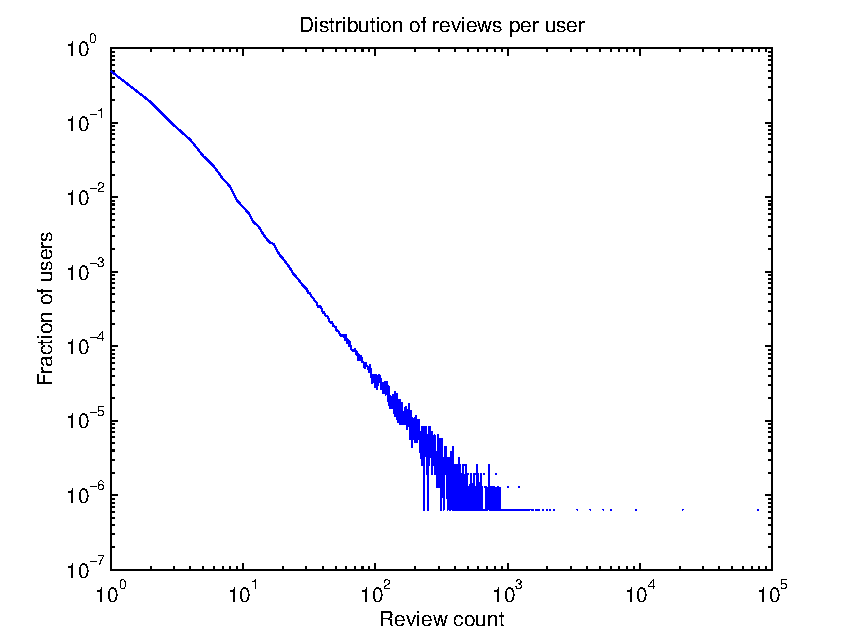
\includegraphics[scale=0.6]{images/user_hist.pdf}
\caption{User review count distribution}
\label{fig:userhist}
\end{figure}

\begin{figure}[h]
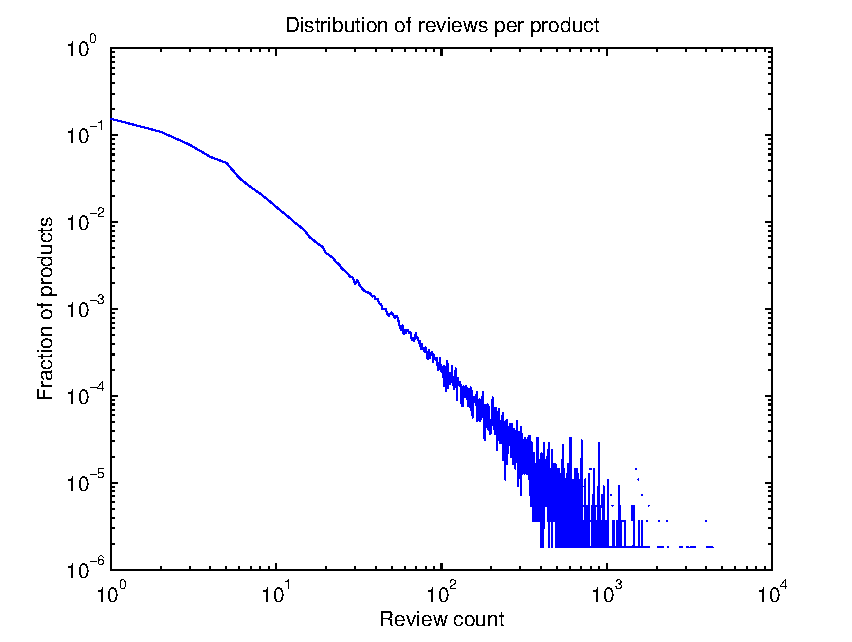
\includegraphics[scale=0.6]{images/product_hist.pdf}
\caption{Product review count distribution}
\label{fig:producthist}
\end{figure}

\begin{figure}[h]
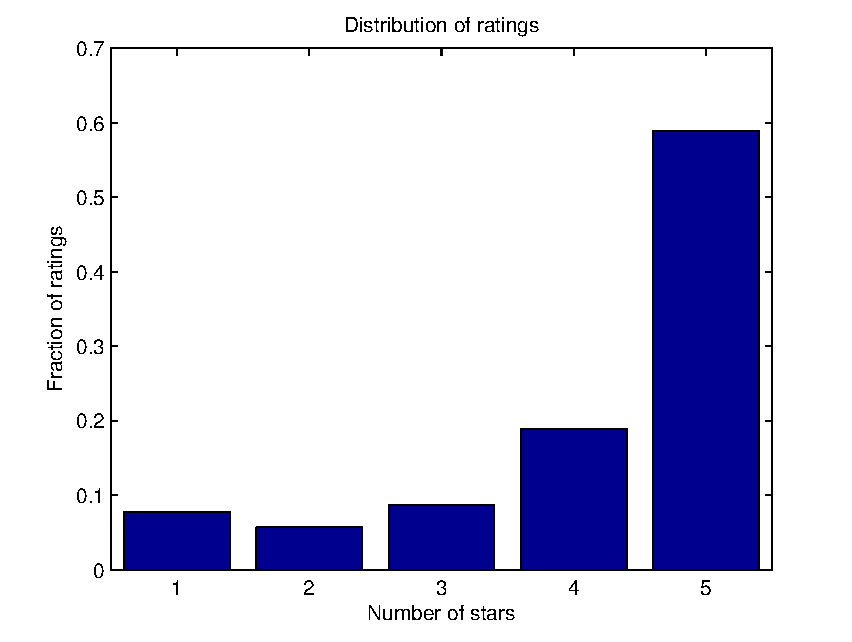
\includegraphics[scale=0.6]{images/ratings.pdf}
\caption{Star rating distribution}
\label{fig:ratings}
\end{figure}


Switching to the Amazon dataset provided several benefits:
\begin{itemize}
\item The number of edges in the graph higher is more one order of magnitude 
higher than in the Yelp dataset.
\item There is no geograhic isolation between groups of users and products
\item The graph is less sparse for users, with a median review count of two 
instead of one
\end{itemize}
For these reasons, we focus this paper mainly on discussions relating to the 
Amazon dataset.

\subsection{Amazon high activity dataset}
The Amazon dataset improves on the Yelp dataset, but it is still fairly 
sparse -- the median user has only 2 reviews. We wanted to experiment on a 
denser dataset to see how density affects model performance. 
As a result, we created a third dataset from a high-activity 
subset of the full Amazon dataset. This dataset comprises all products and 
users with a review count of greater than 5. Though this subset does not 
reflect the real world, it allows us to gain insight on the significance of the 
sparsity problem. The characteristics of this dataset are listed in 
Table~\ref{table:amazonstats_sub}.

\begin{table}[htb]
\centering
\begin{tabular}{|c|c|}
\hline
Users & 89,322 \tabularnewline \hline
Reviews & 3,250,502 \tabularnewline \hline
Products & 174,601 \tabularnewline \hline
Median reviews per user & 14
\tabularnewline \hline
Median reviews per product & 9
\tabularnewline \hline
Average rating given &Mean = 4.11, Median = 5 \tabularnewline
in a review &STD = 1.24
\tabularnewline \hline

\end{tabular}
\caption{ High activity Amazon subset statistics }
\label{table:amazonstats_sub}
\end{table}


%%%%%%%%%%%%%%%%%%%%%%%%%%%%%%%%%%%%%%%%%%%%%%%%%%%%%%%%%%%%%%%%%%%%%%%%%%%%%%%
\section{Models}
\label{sec:models}

We wish to user our models to predict the star rating a given user would 
assign to a given venue or product. To begin, we model our training data as a 
bipartite graph, where each user is connected to an item if the user 
has reviewed
that item. The weight of the edge is the star count associated with that
review. The goal of our model is that for a (user, item) tuple without an
existing review, we will be able to predict the strength of the missing
edge.

In this project, we implement three collaborative filtering algorithms on our 
datasets to solve this modified bipartite graph inference problem. 
Our first model, the neighborhood-based collaborative
filtering approach, focuses on similarity between users. The second model
is item-based collaborative filtering, which utilizes 
similarity among products rated by the same user. Finally, our third model
assumes a hidden similarity layer exists between users and items, and
attempts to learn this using stochastic gradient descent. Further details
about these models are outlined below.

\subsection{Neighborhood-based model}

In this algorithm, we predict ratings for a user based on the known
ratings from similar users. The steps are outlined below:

\begin{enumerate}
  \item For a given user i, calculate similarity between this users and all
    other users. 
  \item Represent the dataset as a sparse matrix of businesses and users, with
    values in the matrix being the ratings assigned by the users to the
    businesses. Take the cosine similarity between the vectors of two users.
  \item Select the k nearest neighbors of i based on this similarity measure
  \item Compute a predicted rating for i based on a weighted combination of the
    nearest neighbors. ratings
\end{enumerate}

While running this model, we sometimes find users with no ratings history 
except for the one rating we are trying to predict, or we find users whose 
neighbors have never rated the product in the prediction. When this happens, we 
have the neighborhood predict a default value of four.

\subsection{Modified neighborhood model}

Given the sparsity of our datasets, we also try a variation of the
neighborhood based collaborative filtering approach, in which instead of
simply selecting the k nearest neighbors for a user, we select the k
nearest neighbors out of those who have rated the product. This works
poorly for items that have fewer than k reviews, as we end up simply
calculating the average of the scores assigned to those items. When no 
neighbors can be found, this algorithm becomes useless, so we skip those 
particular predictions. Our motivation for using this variation is that 
these changes might alleviate the ``cold start'' problem when users have no 
history.

\subsection{Item-based model}

Sarwar, et al.\cite{bib:sarwar} take a item-base collaborative filtering algorithms,
 which, focusing on the similarities between items rather than
users. In a similar vein, we also use the graph structure in the bipartite
graph of users and businesses to compute a similarity metric between
businesses. The motivating intuition is that users are likely to rate
similar businesses comparably, yielding a better prediction for the (user,
business) pair than the neighborhood-based method.

Considering the item-space rather than the user space takes care of some 
crucial problems. Namely, the search for similar users in the
high-dimensional space of user profiles over the large set of all Yelp.s
users is prohibitively computationally expensive. It also partially takes
into account a missing data problem regarding new user profiles that have
comparatively few ratings for businesses.

The steps involved in item-based collaborative filtering are as follows:
\begin{enumerate}
\item When considering the (user, item) pair, calculate similarities between
  the target business and each of the items the user has rated previously
\item Use cosine similarity and use all of the ratings for a particular item
  over the user space as the feature vector to measure similarity between
  items.
\item Look for the k nearest neighbors to the target item from among the set of
  items the user has rated previously
\item Take a weighted average of the selected k items to compute a prediction
  of the rating for the target item
\end{enumerate}

When we encounter examples with no history, we again predict a default value 
of 4, as in the neighborhood-based model.


\subsection{Matrix factorization}

In our final model, we predict ratings by estimating
parameters for statistical models for user ratings. Unlike the previous
two methods which projected user ratings based on user similarity or
item similarity, matrix factorization models assume that a similarity layer
between users and items is induced by a hidden lower-dimensional structure
latently present in the data.

If we associate each item $i$ with a vector $q_i \in R^f$, and each user $u$ with a
vector $p_u \in R^f$, then we can use the resulting dot product $q_i^Tp_u$ to represent
the interest between user $u$ and item $i$.
Here, we are mapping both items and users to a unified Euclidean space
representing the network topology of the bipartite graph.
The problem then turns into a
learning problem where we attempt to learn the distribution vectors for
$q_i,p_u$. From those vectors one can infer the interest that a user will
have in an item from the simple dot product.

A number of methods can be employed to learn these factor vectors for
users and items. In their work on Netflix recommender systems, Bell, et al.
\cite{bib:bellkor} describe possible usage of two common approaches, namely,
stochastic gradient descent and alternating least squares. Given the
sparsity of our training set, stochastic gradient descent is a suitable
option, whereby we compute, at each step, a prediction error $e_{ui}
=r_{ui}-q_i^Tp_u$ for each user-item training pair, and adjust our
parameters $q_i,p_u$ accordingly in the opposite direction of the gradient.


%%%%%%%%%%%%%%%%%%%%%%%%%%%%%%%%%%%%%%%%%%%%%%%%%%%%%%%%%%%%%%%%%%%%%%%%%%%%%%%
\section{Results and Discussion}
\label{sec:results}

In this section, we report the results of our models on the Yelp dataset, 
the full Amazon
dataset and on the Amazon high-activity subset. We count a dataset  
example as a 3-tuple of product, user, and star rating. For each of the three 
datasets, we randomly shuffle the examples and make train-test splits as shown 
in Table~\ref{table:traintest}.

\begin{table}[htb]
\centering
\begin{tabular}{|c|c|c|}
\cline{2-3}

\multicolumn{1}{c|}{}  & {Num train}  & {Num test} \tabularnewline \hline
Yelp & 137154 & 15173 \tabularnewline
Amazon (Full) & 6277889 & 7500 \tabularnewline
Amazon (High activity) & 3246602 & 3900 \tabularnewline
\hline
\end{tabular}
\caption{Train/test splits}
\label{table:traintest}
\end{table}

We measure performance over the test sets using 
root-mean-square error. The errors are normalized by dividing by 4, the maximum 
difference between the highest and lowest star ratings possible. However, 
in the interest of preserving granularity for model comparison, predicted
fractional ratings are not rounded to the nearest integer before calculating 
the errors. 

It should be mentioned that the proportion of test items to train items for 
the Yelp dataset is much higher than for the other two datasets. This is 
because after switching datasets, we felt it was not necessary to test 10\% of 
the dataset, especially when the Amazon graph was much larger. We felt that 
7500 and 3900 test items for two Amazon datasets were sufficient, given that we 
were now working with datasets that took much longer to test. 


%%%%%%%%%%%%%%%%%%%%%%%%%%%%%%%%%%%%%%%%%%%%%%%%%%%%%%%%%%%%%%%%%%%%%%%%%%%%%%%
\subsection{Neighborhood-based model}

\subsubsection{Yelp dataset}
Our first attempt at the neighborhood-based model was on the Yelp dataset. The 
results are shown in Table \ref{table:modelone_yelp} and Figure 
\ref{fig:modelone_yelp}:

\begin{table}[htb]
\centering
\begin{tabular}{|c|c|}
\cline{2-2}

\multicolumn{1}{c|}{}  & {Normalized RMSE} \tabularnewline \hline
$k$ = 1 & 0.3143  \tabularnewline
$k$ = 3 &  0.3149 \tabularnewline
$k$ = 5 & 0.3155  \tabularnewline
$k$ = 10 & 0.3162  \tabularnewline
$k$ = 50  & 0.3189 \tabularnewline
$k$ = 100 & 0.3183 \tabularnewline
$k$ = 1000 & 0.2993 \tabularnewline
\hline
Always predict 4 & 0.3137 \tabularnewline 
Average of all other users & 0.2723 \tabularnewline

\hline
\end{tabular}
\caption{Neighborhood model, Yelp dataset}
\label{table:modelone_yelp}
\end{table}

\begin{figure}[h]
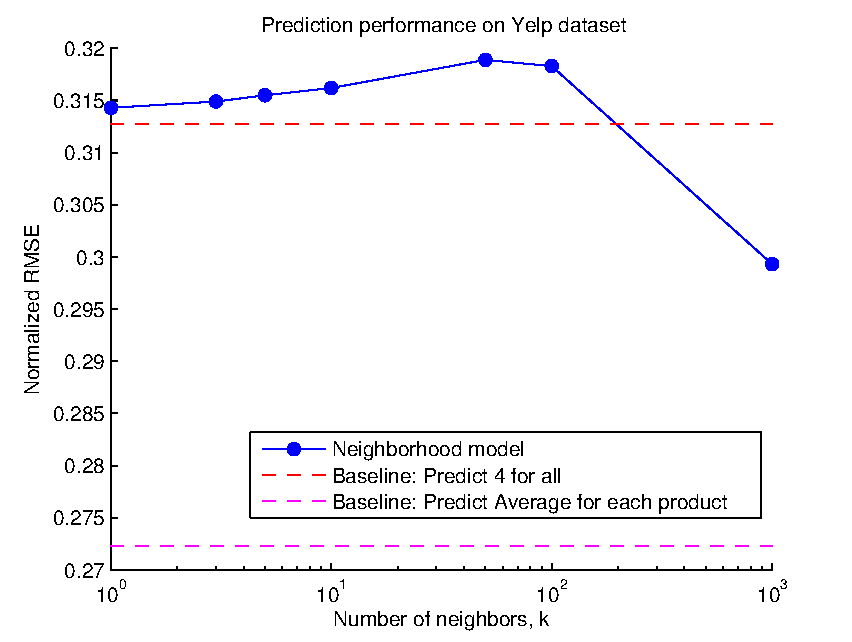
\includegraphics[scale=0.6]{images/modelone_yelp.pdf}
\caption{Neighborhood model, Yelp dataset}
\label{fig:modelone_yelp}
\end{figure}

The neighborhood model's performance on the Yelp dataset is not impressive. The 
model performs better than a baseline model that predicts 4 for every product, 
but not better than another baseline model that predicts the average rating 
given by all other users. 

The error increases with $k$ at first, most likely because adding less similar 
users dilutes the quality of the similar users pool. However, as we increase 
$k$ to over 50, the error decreases again. This means that the model approaches 
the baseline of predicting the average for all users. 

The main problem with the Yelp dataset is its sparsity -- the median review 
count is one, which means that we can expect over half our users in the test 
set to have reviewed only one item. If we try to predict that rating, we 
do not have any other history to go on. Therefore, we cannot find an similar 
users by any reasonable definition, and we just predict a default value of 4. 

Since the neighborhood model is user-based, this lack of similarity between 
users is especially bad. We conclude that the neighborhood approach is not 
effective on the Yelp dataset.

%%%%%%%%%%%%%%%%%%%%%%%%%%%%%%%%%%%%%%%%%%%%%%%%%%%%%%%%%%%%%%%%%%%%%%%%%%%%%%%
\subsubsection{Full Amazon dataset}
Next, we wanted to see if having a larger dataset would change the neighborhood 
model's performance. We tested only $k$ values under 25, since having more 
than 25 neighbors just approaches predicting the average and does not give 
insight about the usefulness of close neighbors. 

The results on the full Amazon dataset 
are shown in Table~\ref{table:modelone_full} and Figure~\ref{fig:modelone_full}.

\begin{table}[htb]
\centering
\begin{tabular}{|c|c|}
\cline{2-2}

\multicolumn{1}{c|}{}  & {Normalized RMSE} \tabularnewline \hline
$k$ = 1 & 0.3497  \tabularnewline
$k$ = 3 &  0.3374 \tabularnewline
$k$ = 5 & 0.3348  \tabularnewline
$k$ = 10 & 0.3262  \tabularnewline
$k$ = 25  & 0.3220  \tabularnewline
\hline
Always predict 4 & 0.3211 \tabularnewline 
Average of all other users & 0.3007 \tabularnewline

\hline
\end{tabular}
\caption{Neighborhood model, full Amazon dataset}
\label{table:modelone_full}
\end{table}

\begin{figure}[h]
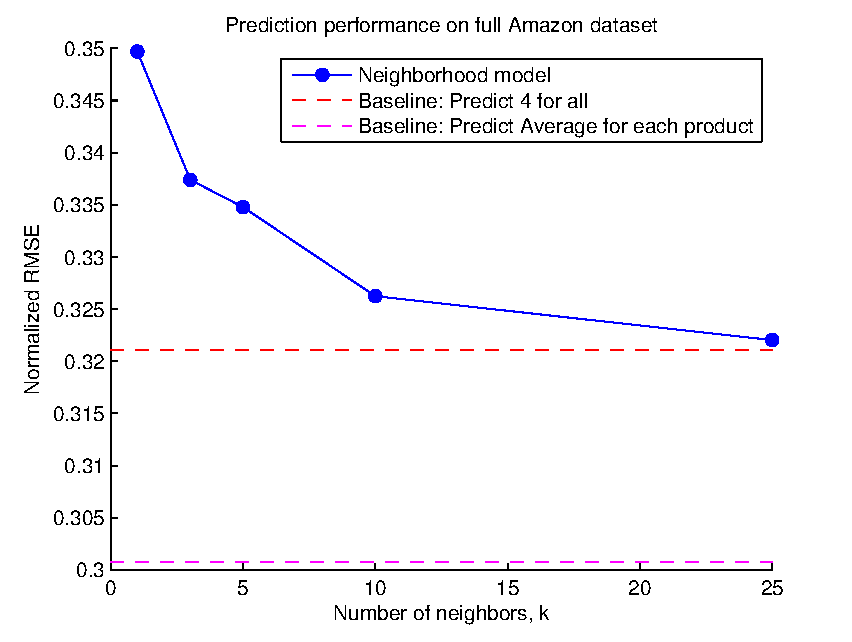
\includegraphics[scale=0.6]{images/modelone_full.pdf}
\caption{Neighborhood model, full Amazon dataset}
\label{fig:modelone_full}
\end{figure}

Even though the Amazon full dataset is much larger than the Yelp dataset, it 
is still quite sparse: the median review count for a user is 2. As a result, 
the Amazon full dataset does not perform any better on this model. 
An interesting thing to note is that this dataset does not seem to have any 
initial rise in error with an increase in neighbors. It starts with the highest 
error at $k = 1$ and declines steadily as we bring more people into the pool. 
This suggests calculating user similarity using cosine similarity is not at all 
helpful on Amazon; an item-based method might fare better. 

Another conclusion we can draw is that sparsity does indeed matter more than 
dataset size. Even though the Amazon dataset is one order of magnitude larger 
than the Yelp dataset, there doesn't seem to be a performance gain because the 
model still does not beat the baselines. 


%%%%%%%%%%%%%%%%%%%%%%%%%%%%%%%%%%%%%%%%%%%%%%%%%%%%%%%%%%%%%%%%%%%%%%%%%%%%%%%
\subsubsection{Amazon high-activity dataset}
To test the sparsity hypothesis further, we ran the neighborhood model on the 
high activity Amazon dataset. The results are shown in 
Table~\ref{table:modelone_subset} and Figure~\ref{fig:modelone_subset}.

\begin{table}[htb]
\centering
\begin{tabular}{|c|c|}
\cline{2-2}

\multicolumn{1}{c|}{}  & {Normalized RMSE} \tabularnewline \hline
$k$ = 1 & 0.1352  \tabularnewline
$k$ = 3 & 0.1380 \tabularnewline
$k$ = 5 &  0.1410 \tabularnewline
$k$ = 10 &  0.1467 \tabularnewline
$k$ = 25  &  0.1549 \tabularnewline
\hline
Always predict 4 & 0.3049 \tabularnewline 
Average of all other users & 0.2513 \tabularnewline
\hline
\end{tabular}
\caption{Neighborhood model, high-activity dataset}
\label{table:modelone_subset}
\end{table}

\begin{figure}[h]
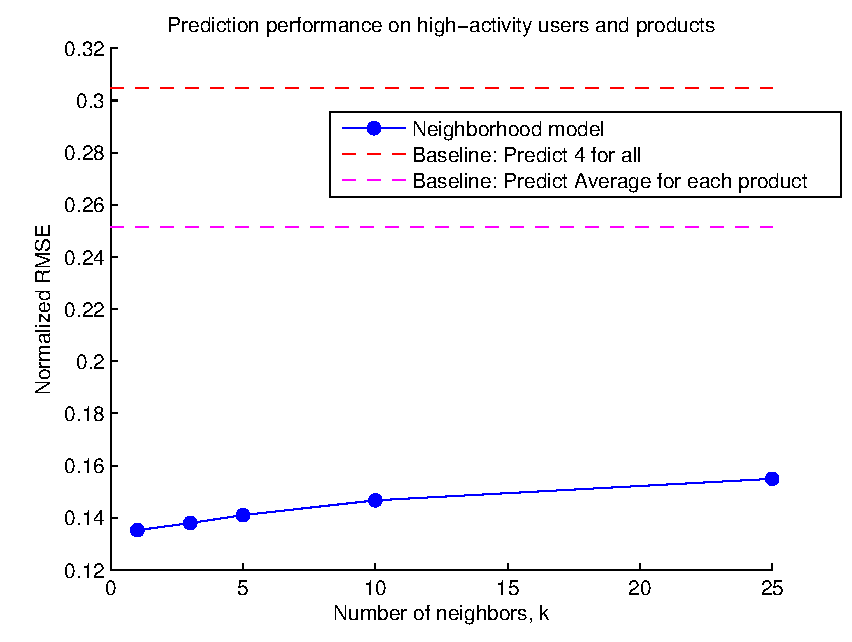
\includegraphics[scale=0.6]{images/modelone_subset.pdf}
\caption{Neighborhood model, high-activity dataset}
\label{fig:modelone_subset}
\end{figure}

The high-activity dataset achieves remarkably good performance. At every value 
of $k$, the model beats both baselines. This confirms our hypothesis that 
sparsity was at fault in the poor results on the Yelp dataset and Amazon full 
dataset.

Furthermore, we see that error rises with $k$, which is opposite to 
the falling shape of the curve in the full Amazon dataset. This indicates that 
the error increases as more neighbors of poorer quality are added, so using the 
nearest neighbors as defined by cosine similarity are indeed valuable. 
This trend is in contrast to the Amazon full dataset, 
where most test users did not have any meaningful history to calculate 
neighbors from, resulting in a poor pool of neighbors. 

\subsubsection{Summary of neighborhood models}
In these models, we learned that the user-similarity approach of neighborhood 
models does not work well in sparse datasets where users have few edges. 
Unfortunately, most large datasets are sparse, so it is unlikely that we will 
see good performance from the neighborhood model like in the Amazon high 
activity dataset. Another unattractive quality of the neighborhood model is 
that it is slow. Although there is no training involved, we need to calculate 
user $u$'s similarity with all other users at test time. This is a 
time-expensive procedure unless we store all pairs of similarities 
ahead of time. Based on its poor accuracy and speed, the neighborhood-based 
model is not the best choice to be used alone in a recommendation engine.


%%%%%%%%%%%%%%%%%%%%%%%%%%%%%%%%%%%%%%%%%%%%%%%%%%%%%%%%%%%%%%%%%%%%%%%%%%%%%%%
\subsection{Item-based model}

%%%%%%%%%%%%%%%%%%%%%%%%%%%%%%%%%%%%%%%%%%%%%%%%%%%%%%%%%%%%%%%%%%%%%%%%%%%%%%%
\subsubsection{Full Amazon dataset}
The results of the item-based model on the full Amazon dataset 
are shown in Table~\ref{table:modeltwo_full} and Figure~\ref{fig:modeltwo_full}.

\begin{table}[htb]
\centering
\begin{tabular}{|c|c|}
\cline{2-2}

\multicolumn{1}{c|}{}  & {Normalized RMSE} \tabularnewline \hline
$k$ = 1 & 0.1972 \tabularnewline
$k$ = 3 & 0.2099 \tabularnewline
$k$ = 5 & 0.2185 \tabularnewline
$k$ = 10 & 0.2284 \tabularnewline
$k$ = 25 & 0.2339 \tabularnewline
\hline
Always predict 4 & 0.3211 \tabularnewline 
Average of all other users & 0.3007 \tabularnewline

\hline
\end{tabular}
\caption{Item-based model, full Amazon dataset}
\label{table:modeltwo_full}
\end{table}

\begin{figure}[h]
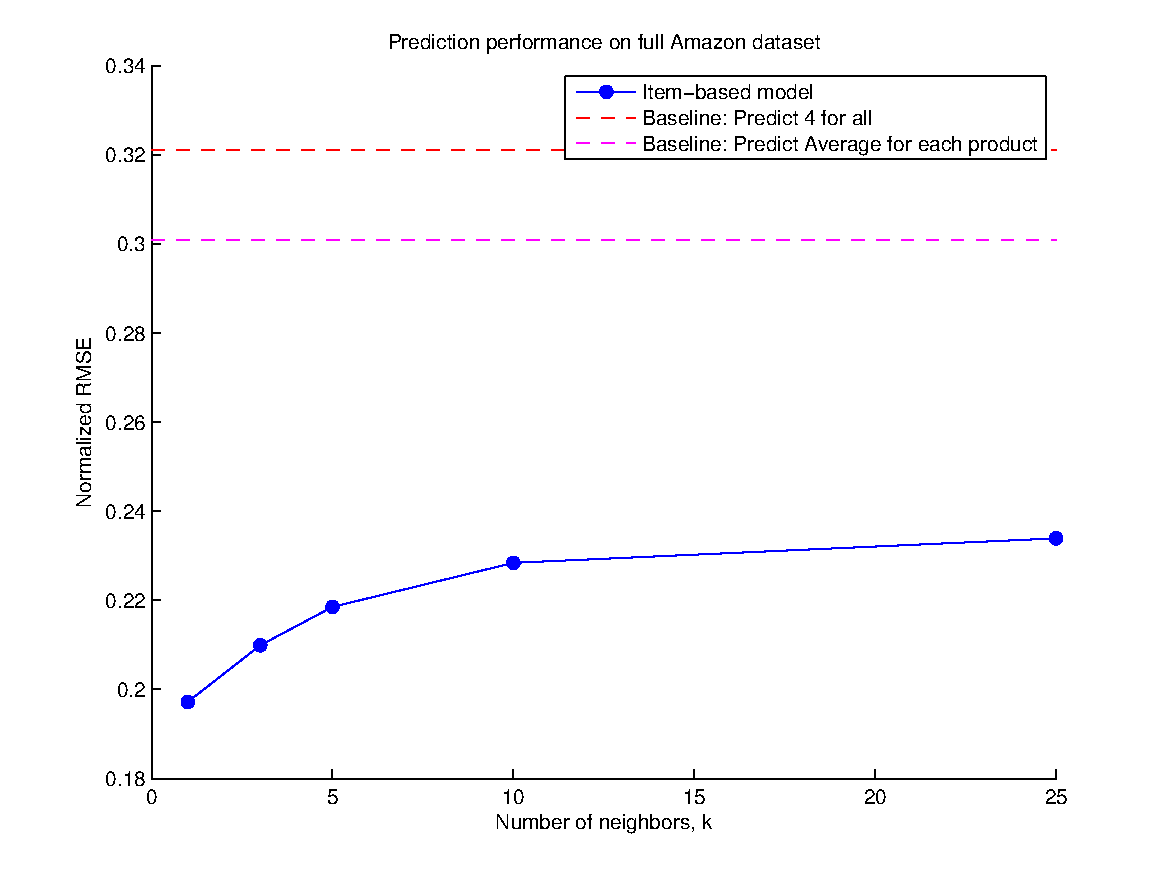
\includegraphics[scale=0.5]{images/modeltwo_full.pdf}
\caption{Item-based model, full Amazon dataset}
\label{fig:modeltwo_full}
\end{figure}

Compared to the neighborhood-based model, the item based model performs
far better on the full dataset. Prior work has stated that item-based
models were specifically created for sparser datasets
\cite{bib:amazon}. One possible explanation for this is that users with
several reviews are likely to have a wider range of ratings; on the other
hand, a user with only two or three reviews is likely to have bestowed the
same rating upon all items he or she has reviewed. As a result, when
trying to make a prediction in a sparse context, it is far more useful to
consider the small number of ratings provided by the user in question,
rather than trying to use this limited set of ratings to find similar
users and make a prediction based on them.
Interestingly, the performance of the model decreases with higher values
of k. This can also be accredited to the previous explanation: a larger
variety of ratings for a user would imply more diversity in ratings. While
the predictions remain the same for low activity users, they get 
worse for those with a lot of ratings. With smaller values of k, we are
averaging over ratings of a few products which are similar to the one in
question; with larger values, we are looking at a whole array of ratings,
which for high activity users is bound to be very diverse, rendering the
average score less useful.


%%%%%%%%%%%%%%%%%%%%%%%%%%%%%%%%%%%%%%%%%%%%%%%%%%%%%%%%%%%%%%%%%%%%%%%%%%%%%%%
\subsubsection{Amazon high-activity dataset}
The results of the item-based model on the high activity Amazon dataset 
are shown in Table~\ref{table:modeltwo_subset} and 
Figure~\ref{fig:modeltwo_subset}.

\begin{table}[htb]
\centering
\begin{tabular}{|c|c|}
\cline{2-2}

\multicolumn{1}{c|}{}  & {Normalized RMSE} \tabularnewline \hline
$k$ = 1 & 0.3636 \tabularnewline
$k$ = 3 & 0.3172 \tabularnewline
$k$ = 5 & 0.3083 \tabularnewline
$k$ = 10 & 0.3024 \tabularnewline
$k$ = 25 & 0.2967 \tabularnewline
\hline
Always predict 4 & 0.3049 \tabularnewline 
Average of all other products & 0.2834 \tabularnewline
\hline
\end{tabular}
\caption{Item-based model, high-activity dataset}
\label{table:modeltwo_subset}
\end{table}

\begin{figure}[h]
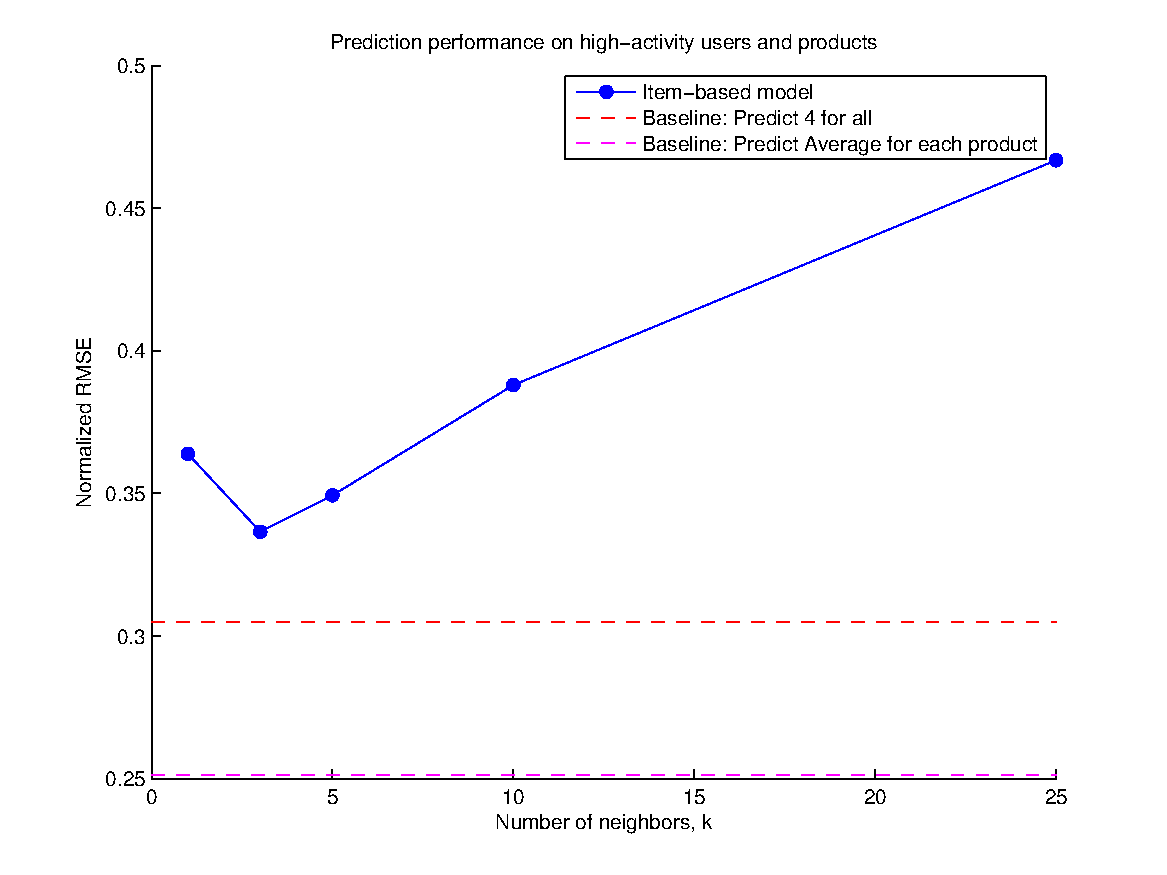
\includegraphics[scale=0.5]{images/modeltwo_subset.pdf}
\caption{Item-based model, high-activity dataset}
\label{fig:modeltwo_subset}
\end{figure}


As expected, the performance of the item-based model decreases in the case
of the less sparse, high-activity dataset. While the neighborhood model
performed a lot better in this context, the item-based model falters, as
it is now predicting averages over more diverse rating sets. The
phenomenon of the low activity user with the same rating for all two or
three rated products no longer exists, removing the boost in prediction
the item-based model received in the sparser dataset.

Additionally, the performance of the model improves with an increase in
the value of k from 1 to 3, and stays fairly stable thereafter. This can
be explained by the fact that each user in this dataset has rated several
products, and basing their rating on one similar product alone may not be
enough, or may be too extreme. When averaging out over a few related
products, the performance therefore increases. Unlike the sparse dataset,
however, there is no help from low activity users for low values of k.


%%%%%%%%%%%%%%%%%%%%%%%%%%%%%%%%%%%%%%%%%%%%%%%%%%%%%%%%%%%%%%%%%%%%%%%%%%%%%%%

\subsection{Matrix factorization}
The last model we tried was matrix factorization. When we ran this model on the 
sparser Yelp and Amazon full datasets, gradient minimization was unable to 
converge. Because the time of each iteration was too long, and there were too 
many parameters to consider, we focused on running this model on the 
high-activity Amazon dataset.

\subsubsection{Amazon high-activity dataset}
The results of matrix factorization are shown in 
Table~\ref{table:modelthree_subset} and
Figure~\ref{fig:modelone_subset}. We varied the number of latent dimensions ($f$)
in the user-product space to take into account overfitting effects. 

\begin{table}[htb]
\centering
\begin{tabular}{|c|c|}
\cline{2-2}

\multicolumn{1}{c|}{} & {Normalized RMSE} \tabularnewline \hline
$f$ = 10 & 0.2231 \tabularnewline
$f$ = 20 & 0.2280 \tabularnewline
\hline
Always predict 4 & 0.3049 \tabularnewline 
Average of all other users & 0.2513 \tabularnewline
\hline
\end{tabular}
\caption{Matrix factorization model, high-activity dataset}
\label{table:modelthree_subset}
\end{table}

\begin{figure}[h]
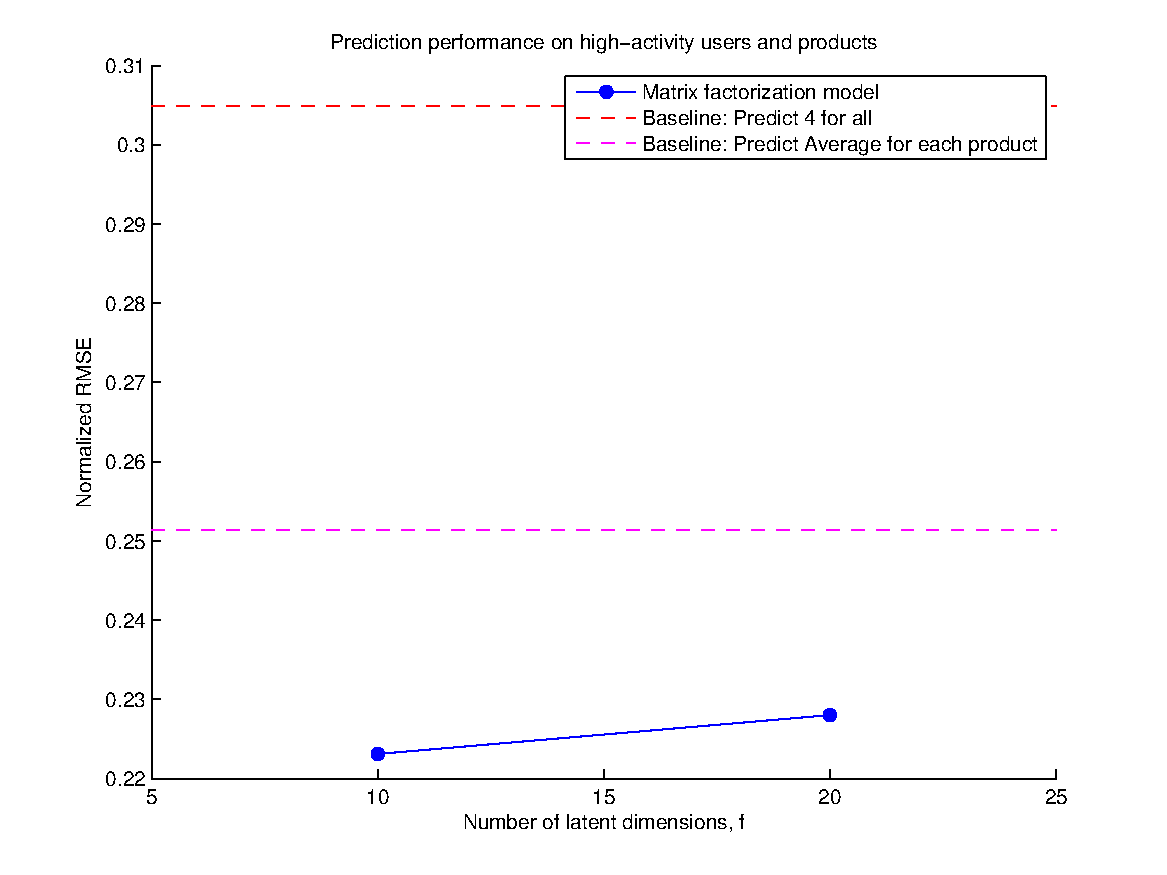
\includegraphics[scale=0.5]{images/modelthree_subset.pdf}
\caption{Matrix factorization model, high-activity dataset}
\label{fig:modelthree_subset}
\end{figure}

This model does fairly well on the high-activity dataset, beating 
both the baselines, though it does not perform as well as the neighborhood 
model. 

As we suspected, a smaller number of latent dimensions raised the RMSE on the 
training set but reduced it on the test set. We did not use regularization in 
this model, so perhaps the model suffers from a bit of overfitting at 
$f = 20$.

It is worth noting that though we tried to run this model with the 
regularization as mentioned in matrix factorization papers 
\cite{bib:matrixfact}, our model performed very poorly with regularization. 
While the purpose of regularization is to avoid overfitting effects by 
penalizing large parameter values, even very small values 
of $\lambda$ (about $10^{-4}$) ended up interfering a great deal with gradient 
descent. As a result, in our final factorization method implementation,
we ended up excluding regularization altogether.

If we had more time and more computational power, we would try to increase 
the number of dimensions even more, at least into the hundreds. We would also 
experiment with different regularization values, because perhaps the correct 
combination of $f$ and $\lambda$ is something we have not searched over yet. 
However, this task is currently unfeasible on the Corn machines because of 
memory requirements for high $f$. The timeframe of trying each combination is 
also quite costly, which led us to have only two successful trials. We believe 
the potential of this model is still largely unexplored after this set of 
experiments. 

In a recommendation system, an attractive characteristic of matrix 
factorization is its speed in making predictions. Though training is costly, 
a prediction just involves taking a dot product. However, the disadvantage is 
that new users and products are hard to add, as this would change the 
dimensions of the matrix. 

%%%%%%%%%%%%%%%%%%%%%%%%%%%%%%%%%%%%%%%%%%%%%%%%%%%%%%%%%%%%%%%%%%%%%%%%%%%%%%%
\section{Conclusion}
In this project, we built three models for ratings prediction:
\begin{enumerate}
\item The neighborhood model predicts ratings based on ratings from similar 
users. We found that this approach performs very poorly on sparse data and is 
also slow due to the calculation of user similarity at test time.

\item The item-based model makes predictions based on item similarity. Its 
advantage is that product similarity can be calculated offline, and the system 
is less dependent on changes in users. 

\item The matrix factorization model learns latent parameters for products and 
users. In our experiments, the model had promising results on the high-activity 
dataset, but was too slow for much further experimentation. Though training is 
slow, a trained model can make predictions quickly by taking a dot product. 

All three collaborative filtering models suffer from the ``cold start'' 
problem, in which users with little or no history have no basis for prediction. 
To address this problem, it would help to combine collaborative filtering with 
content-based filtering, in which users and products have hand-annotated 
descriptions. This would make for an exciting extension to our current project. 
In fact, many of the real-world recommendation systems today 
already use complex and interesting combinations of the techniques in this 
paper.

\end{enumerate}

\begin{thebibliography}{99}

\bibitem{bib:recsys}
Adomavicius, G., Tuzhilin, A. (2005). Toward the next generation of recommender systems: a survey of the state-of-the-art and possible extensions. Knowledge and Data Engineering, IEEE Transactions on , 17(6),  734- 749.

\bibitem{bib:matrixfact}
Bell, R., Koren, Y., Volinsky, C. (2009). Matrix factorization techniques for recommender systems. IEEE Computer 42(8):30-37

\bibitem{bib:bellkor}
Bell, R., Koren, Y., Volinsky, C. (2009). 
The BellKor solution to the Netflix Prize. Technical Report, AT\&T Labs 
Research, 2007b. 
http://www.netflixprize.com/assets/ProgressPrize2007\_KorBell.pdf


\bibitem{bib:tapestry}
Goldberg, D., Nichols, D., Oki, B., Terry, D. (1992). 
Using collaborative filtering to weave an information tapestry. 
Communications of the Association of Computing Machinery, 35(12), 61-70.

\bibitem{bib:amazon}
Linden, G., Smith, B., York, J. (2003). Amazon.com recommendations: Item-to-item collaborative filtering. IEEE Internet
Computing, 7(1), 76-80.

\bibitem{bib:recsys2}
Melville, P., Sindhwani, V. (2010).
Recommender Systems. The Encyclopedia of Machine Learning. 
http://www.prem-melville.com/publications/recommender-systems-eml2010.pdf

\bibitem{bib:sarwar}
Badrul Sarwar, George Karypis, Joseph Konstan, and John Reidl. 2001.
Item-based collaborative filtering recommendation algorithms.
In Proceedings of the 10th international conference on World Wide Web (WWW '01). ACM, New York, NY, USA, 285-295. 

\end{thebibliography}

\section{Acknowledgments}
We would like to acknowledge Jure Leskvec and the teaching staff of 
Stanford's CS224W for their advice and support. We also thank Yelp for the 
Yelp Academic Dataset, and Jure Leskovec for the Amazon dataset.

\end{document}
